\subsubsection{Word Mover's Distance} % (fold)
\label{sub:own_wmd}
Finally, we used the Word Mover's Distance which was also implemented in the gensim library. To do so, it was also necessary to create word embeddings for our requirement sentences first. Again, we could use the word vectors of the aforementioned word2vec models. Instead of basing our clusters on the distance between word vectors though, we could now calculate a distance matrix which holds the calculated Word Mover's Distance from every sentence to every other sentence, as represented in \autoref{tbl-wmd-matrix}. Note how the Word Mover's Distance is symmetric. So the distance to travel from $s_1$ to $s_2$ is the same as if your travelling vice versa.

\begin{table}[ht]
\centering
\begin{tabular}{lllll}
             & $s_1$                      & $s_2$                      & $s_3$                      & ...                      \\ \cline{2-5} 
\multicolumn{1}{l|}{$s_1$} & \multicolumn{1}{l|}{0}    & \multicolumn{1}{l|}{0.83} & \multicolumn{1}{l|}{3.23} & \multicolumn{1}{l|}{...} \\ \cline{2-5} 
\multicolumn{1}{l|}{$s_2$} & \multicolumn{1}{l|}{0.83} & \multicolumn{1}{l|}{0}    & \multicolumn{1}{l|}{2.77} & \multicolumn{1}{l|}{...} \\ \cline{2-5} 
\multicolumn{1}{l|}{$s_3$} & \multicolumn{1}{l|}{3.23} & \multicolumn{1}{l|}{2.77} & \multicolumn{1}{l|}{0}    & \multicolumn{1}{l|}{...} \\ \cline{2-5} 
\multicolumn{1}{l|}{...}  & \multicolumn{1}{l|}{...}  & \multicolumn{1}{l|}{....} & \multicolumn{1}{l|}{...}  & \multicolumn{1}{l|}{0}   \\ \cline{2-5} 
\end{tabular}
\caption{Sentence Matrix containing the Word Mover's Distance from one sentence to another}\label{tbl-wmd-matrix}
\end{table}

 Since by its nature, the resulting matrix already was a 2-dimensional array with equal dimensions, it was not necessary anymore to perform any further reduction. We could use this matrix instead to directly create some clusters using K-Means.

 \begin{figure}[ht]
  \begin{center}
    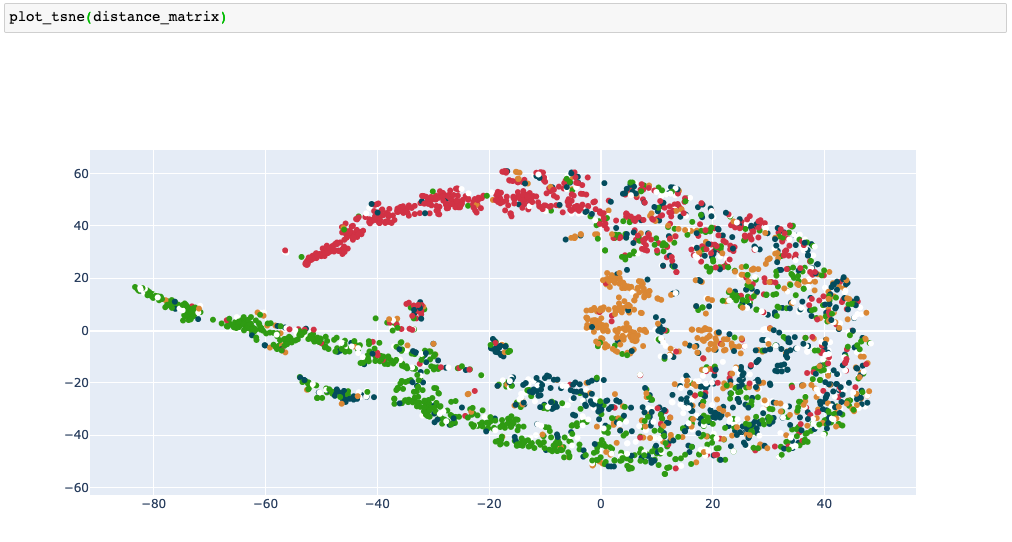
\includegraphics[width=\textwidth]{screenshots/our_word_movers_distance_tsne.png}
    \caption{Distance Matrix of the Word Mover's Distance with a self-trained model (plotted with t-SNE)}
    \label{fig:wmd-selftrained-1}
  \end{center}
\end{figure}
\FloatBarrier